

由于软件的运行性能和处理器的结构有着非常紧密的联系,所以本节首先介绍龙芯3号系列处理器的硬件体系特点,为后续章节的优化工作做出理论基础。

\subsection{龙芯3号处理器架构介绍\cite{Loongson3A-Manual}}

龙芯3号的可伸缩互连结构如下图\ref{fig:Loongson3-System-Struct}所示。在图中,龙芯3号片内采用二维mesh互连结构,其中每个结点由8*8的交叉开关组成,每个交叉开关连接四个处理器以及分成四个体的共享二级Cache,并与东(E)南(N)西(W)北(N)四个方向的其他结点互连。因此,2*2的mesh可以连接16个处理器,4*4的mesh可以连接64个处理器。龙芯3号的互连网络采用128位支持Cache一致性的AXI(AMBA3.0)标准接口。

\begin{figure}[H] 
  \centering
  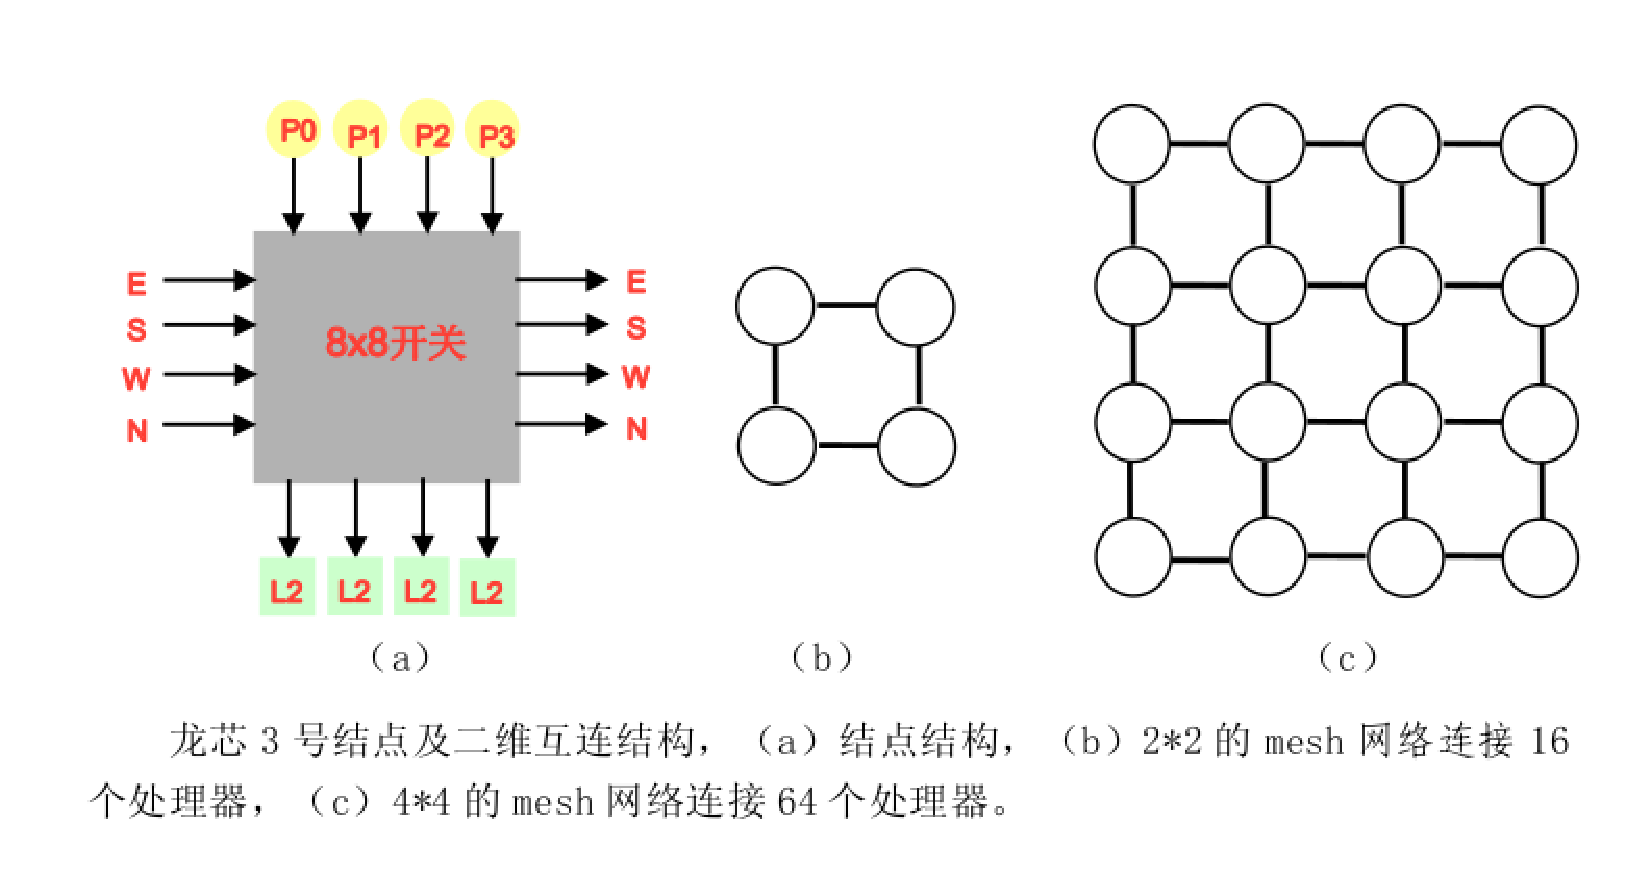
\includegraphics[width=10cm,height=6cm]{figures/chap02/Loongson3-System-Struct}
  \caption{龙芯3号系统结构}
  \label{fig:Loongson3-System-Struct}
\end{figure}

龙芯3号的片内二级Cache分布在不同的结点中,被片内的所有处理器共享。每个结点的二级Cache根据地址分成interleave的四个体,可以被并行访问。所有结点的二级Cache统一编址,每个Cache块都有一个固定的home结点,并在home结点处维护相应Cache块的目录,通过基于目录的Cache一致性协议维护一级Cache的一致性。每个结点(或多个相邻结点)对应一个DDR2内存控制器。内存地址分布和二级Cache的地址分布一致,以简化二级Cache和内存之间的通路并降低二级Cache访问失效的延迟。龙芯3号的IO控制器在边界结点上,通过边界结点空闲的交叉开关端口接入。龙芯3号的IO端口采用 HyperTransport(简称HT)协议。

龙芯3号的一般性结点结构如下图\ref{fig:Loongson3-Node-Struct}所示。每个结点有两级AXI交叉开关连接处理器、二级Cache、内存控制器以及IO控制器。其中第一级AXI交叉开关(称为X1 Switch,简称 X1)连接处理器和二级Cache,通过对AXI的扩充传递跟维护Cache一致性有关的信息。第二级交叉开关(称为X2 Switch,简称X2)连接二级Cache和内存控制器,采用标准的128位AXI协议。

\begin{figure}[H] 
  \centering
  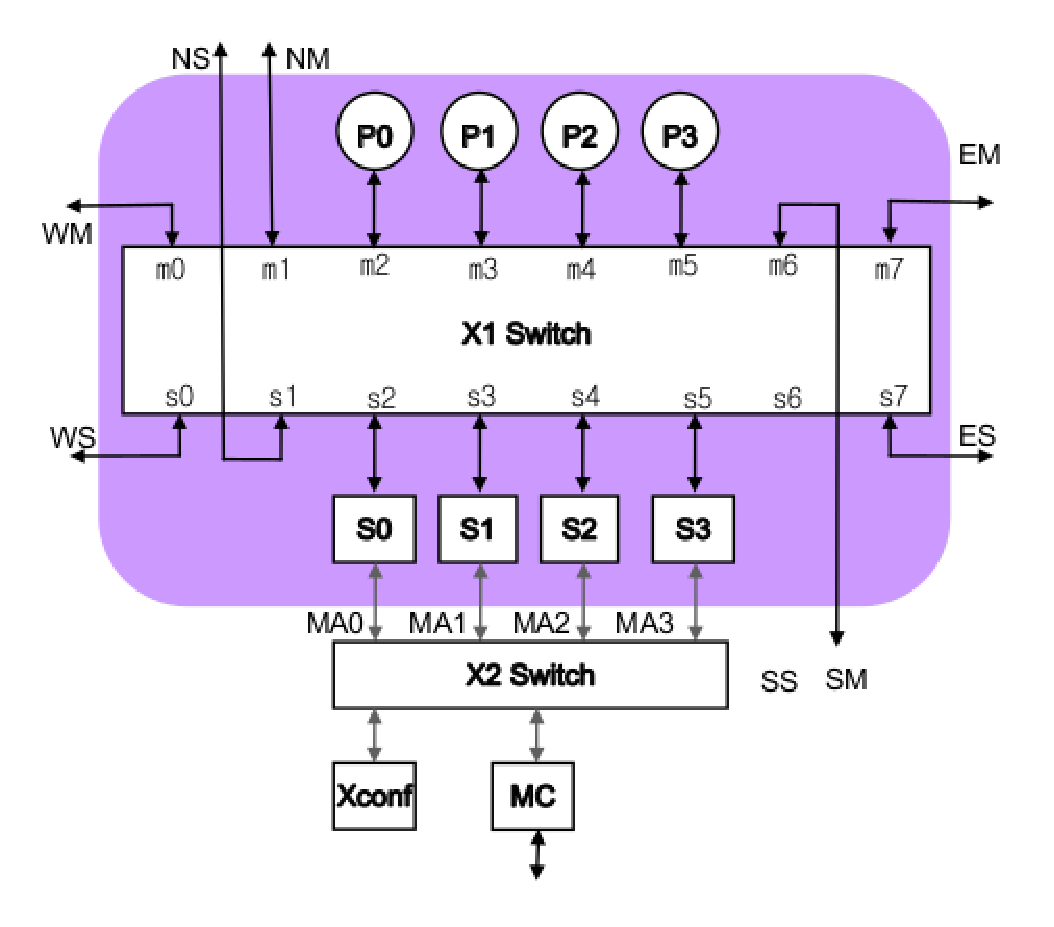
\includegraphics[width=10cm,height=6cm]{figures/chap02/Loongson3-Node-Struct}
  \caption{龙芯3号节点结构}
  \label{fig:Loongson3-Node-Struct}
\end{figure}

在每个结点中,最多8*8的X1交叉开关通过四个Master端口连接四个GS464处理器核(图中 P0、P1、P2、P3),通过四个Slave端口连接统一编址的四个 interleave二级Cache块(图中 S0、S1、S2、S3),通过四对Master/Slave端口连接东、南、西、北四个方向的其他结点或IO结点(图中 EM/ES、SM/SS、WM/WS、NM/NS)。

X2交叉开关通过四个Master端口连接四个二级Cache块,至少一个Slave端口连接一个内存控制器,至少一个Slave端口连接一个交叉开关的配置模块(Xconf)用于配置本结点的X1和X2的地址窗口等。还可以根据需要连接更多的内存控制器和IO端口等。

在龙芯3号的互连系统只是定义上层协议,会不对传输协议的实现做具体规定,因此,结点之间的互连即可以采用片上网络进行实现,也可以通过I/O控制链路实现多芯片的互连。在一个4结点16核系统为例,既可以通过4片4核芯片组成,也可以通过2片8核芯片,或基于一个单芯片4节点16核芯片组成。由于互连系统的物理实现对软件透明,上述3种配置的系统可以运行相同的操作a系统进行。

\subsection{龙芯3号平台Radeon显卡介绍}

在龙芯3号系列处理是平台上常用到的显卡设备就是Radeon系列显卡,本文的Mesa3D硬件加速相关的优化都是基于Radeon系列显卡实现的,所以这里对该系列显卡做简单的介绍。

\subsubsection{Radeon显卡命令处理机制}
Radeon显卡提供驱动使用命令流(Command Stream)的形式进行对显卡编程:驱动程序将需要对显卡进行配置的一连串命令写入命令缓冲区,写完之后进入让出处理器,显卡按照命令写入的顺序执行这些命令,执行完成后触发中断通知驱动。具体来说就是CPU将这些命令放入一个称为命令环的环形缓冲区中,命令环是GTT内存中分出来的一片内存,驱动程序往命令环中填充命令,填充完后通知GPU已经写入命令,接着GPU的命令处理器CP(Command Processor)接收并解析驱动程序发送过来的命令流,将解析后的数据传输给图形控制器的其他模块,包括3D图形处理器、2D图形处理器、视频处理器。

\begin{figure}[H] 
  \centering
  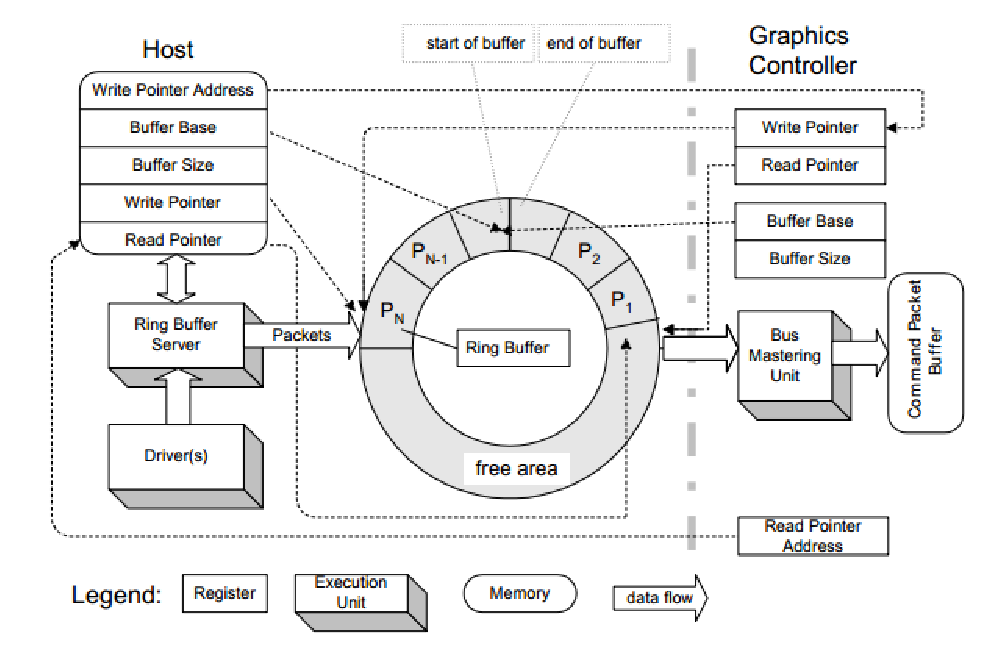
\includegraphics[width=10cm,height=6cm]{figures/chap02/CommandBuffer}
  \caption{Radeon显卡命令处理机制}
  \label{fig:CommandBuffer}
\end{figure}

\subsubsection{Radeon显卡3D图形渲染管线}

Radeon系列显卡通过内置的3D图形流水线帮助实现图形渲染的硬件加速,这里以Radeon R600显卡为例介绍其内部的图形流水线结构。

\begin{figure}[H] 
  \centering
  \includegraphics[width=9cm,height=10cm]{figures/chap02/R600-Pipeline}
  \caption{R600图形渲染管线}
  \label{fig:R600-Pipeline}
\end{figure}

如图\ref{fig:R600-Pipeline}所示,输入数据大体上按照“顶点处理”、“图元组装”、“光栅化”、“片段处理”、“输出”的过程流经图形硬件。这些阶段几乎完全覆盖了前面图\ref{fig:OpenGL-Pipeline}里面的渲染过程,更加详细信息可查阅参考文献Radeon R6xx/R7xx Acceleration\cite{Radeon-Manual}。
